% ============================================================================
% GFD: decoding mass from observed rotation curves (no dark matter halo)
% Figures: fig1_mw_m33, fig2_ngc3198 (generated by generate_letter_figures.py).
% ============================================================================
\documentclass[aps,twocolumn,amsmath,amssymb,reprint,nofootinbib,nobalancelastpage]{revtex4-2}

\usepackage{graphicx}
\usepackage[hidelinks]{hyperref}
\usepackage{url}

% Single clean rule above references (revtex default can render as thick/double)
\makeatletter
\renewcommand{\bibsection}{%
  \par\vspace{1ex}%
  \noindent\rule{\linewidth}{0.4pt}%
  \par\vspace{0.5em}%
}
\makeatother

\begin{document}

\title{Gravity Field Dynamics: Decoding mass from observed rotation curves}

\author{Stephen Nelson}
\email{stephen@fielddynamics.org}
\affiliation{Field Dynamics Research, ORCID: 0009-0008-6190-3269}

\date{February 2026}

% ----------------------------------------------------------------------------
% ABSTRACT
% ----------------------------------------------------------------------------
\begin{abstract}
\vspace{1.2\baselineskip}
Galaxy rotation curves imply more mass than Newtonian gravity and visible matter predict. Two standard responses are dark matter halos (with parameters fitted per galaxy) and modified gravity such as MOND; neither offers a way to go from observed velocity to implied mass without assuming a mass model. We present a framework based on tetrad gravity and ghost-free bimetric gravity, with two field equations that are algebraically invertible: the same equations that give rotation velocity from mass also give enclosed mass from velocity. Applied to the Milky Way and M33 with no fitted gravitational parameters (only the constants $G$ and $a_0$), the inverse pipeline yields enclosed mass profiles that match independently inferred baryonic mass to within a factor of order unity, with no dark matter halo. We do not fit a mass model to the rotation curve; we transform observed velocity into enclosed mass using the same bidirectional covariant (the field equations that run both ways) that defines the theory.
\end{abstract}

\maketitle

% ----------------------------------------------------------------------------
% 1. INTRODUCTION
% ----------------------------------------------------------------------------
\section{Introduction}
\label{sec:intro}

The circular velocity of gas and stars as a function of radius, the rotation curve, is one of the best-measured properties of disk galaxies. In Newtonian gravity, that curve implies an enclosed mass at each radius. When the curve stays flat at large radii, the implied mass grows without bound unless one invokes unseen matter. That is the mass discrepancy: rotation curves suggest more mass than we see.

Two standard approaches address it. In the first, dark matter halos are added; their density profiles (e.g., Navarro-Frenk-White, NFW) are fitted to each galaxy, introducing concentration, scale radius, and virial mass. In the second, the force law is modified (e.g., MOND); the rotation curve is then predicted from an assumed baryonic mass distribution, but there is no algebraic way to run the equations in reverse. Given only the observed velocities, neither approach yields an enclosed mass profile without further assumptions.

We present a framework in which the field equations go both ways. Given a mass distribution, the equations predict the rotation curve. Given a rotation curve, the same equations yield the enclosed mass, with no mass model and no halo parameters. The only inputs are the observed radii and velocities and two constants: Newton's constant $G$ and an acceleration scale $a_0 = 1.2\times10^{-10}$~m/s$^2$ (standard value \cite{Milgrom83}). We apply this pipeline to the Milky Way and M33 and show that the mass implied by the inverse transformation lands near the baryonic mass (the mass in stars and gas) and far below the mass required by a dark matter halo fit. The velocity curves look similar across frameworks; the mass implications do not.

% ----------------------------------------------------------------------------
% 2. FRAMEWORK
% ----------------------------------------------------------------------------
\section{Framework}
\label{sec:framework}

The framework is based on the tetrad formalism of general relativity (\cite{mtw1973,wald1984}) and ghost-free bimetric gravity (\cite{hassan2012}). The governing relations are the Poisson equation and the transition relation; we apply them in the spherically symmetric case (appropriate for rotation curves). We state these equations and apply them to the inverse pipeline; their derivation from the full covariant theory is beyond the scope of this letter.

\paragraph{Part 1: Poisson equation.}
The potential satisfies the standard Poisson equation
\begin{equation}
\nabla^2 \Phi = 4\pi G\,\rho
\label{eq:poisson}
\end{equation}
with $G$ the Newtonian gravitational constant (CODATA). The equation introduces no free parameters beyond $G$.

\paragraph{Part 2: Transition between source and total acceleration.}
The acceleration that governs orbits is not the Newtonian value alone. A scalar-tensor extension modifies it. The action is
\begin{equation}
\begin{split}
S_{\mathrm{ST}} = \int d^4 x\,\sqrt{-g}\,\bigg[ \frac{R}{16\pi G} - \frac{a_0^2}{8\pi G}\,F\big(|\nabla\Phi|^2/a_0^2\big)
\\
- \frac{1}{4}\,e^{-2\Phi/c^2}F_{\mu\nu}F^{\mu\nu} + \mathcal{L}_{\mathrm{matter}} \bigg].
\end{split}
\label{eq:action}
\end{equation}
The kinetic term $F$ yields, in the spherically symmetric limit, a relation between the source acceleration $g_{\mathrm{s}}$ (the acceleration implied by the mass distribution via Eq.~\ref{eq:poisson}) and the total acceleration $g_{\mathrm{t}}$ that governs circular orbits. That relation takes the form of the constitutive law $\mu(x) = x/(1+x)$ with $x = g_{\mathrm{t}}/a_0$, familiar in MOND as the so-called simple interpolating function and widely used for rotation-curve fits. Here it is determined by the action rather than chosen. Thus
\begin{align}
g_{\mathrm{t}} &= \frac{g_{\mathrm{s}} + \sqrt{g_{\mathrm{s}}^2 + 4\,g_{\mathrm{s}}\,a_0}}{2}, \\
g_{\mathrm{s}} &= \frac{g_{\mathrm{t}}^2}{a_0 + g_{\mathrm{t}}}.
\label{eq:transition}
\end{align}
At high acceleration, $g_{\mathrm{t}} \to g_{\mathrm{s}}$ (Newtonian). At low acceleration, $g_{\mathrm{t}} \to \sqrt{g_{\mathrm{s}}\,a_0}$. The algebraic form of $F(X)$ that produces Eq.~\ref{eq:transition} from the variational principle is determined by the theory. These relations are used in this letter for the inverse pipeline; the framework rests on these two equations and the constants $G$ and $a_0$, and no other gravitational parameters are introduced.

\paragraph{Inverse pipeline.}
Because both relations are algebraic in the spherical case, we can invert them. Substituting the kinematic acceleration $g_{\mathrm{t}} = v^2/r$ into Eq.~\ref{eq:transition} and the Poisson equation yields a single, closed-form expression for the enclosed mass:
\begin{equation}
M_{\mathrm{enc}}(r) = \frac{r\,v^4}{G\,(a_0\,r + v^2)}.
\label{eq:Menc}
\end{equation}
There is no iteration and no mass model fitting. The rotation curve and the mass profile are two views of the same field: measure one, you infer the other.

% ----------------------------------------------------------------------------
% 3. DEMONSTRATION
% ----------------------------------------------------------------------------
\section{Demonstration}
\label{sec:demonstration}

We apply the framework to the Milky Way and M33. The data are published rotation curves (radii and velocities only). The baryonic mass models are taken from the literature and are not tuned to the rotation curve in this work.

\paragraph{Forward: mass to velocity.}
We use published baryonic models: for the Milky Way, an exponential disk with $M_{\mathrm{disk}} = 7.52\times10^{10}\,M_\odot$ and scale length $R_{\mathrm{d}} = 2.79$~kpc (bulge omitted; at the radii shown the disk dominates~\cite{McMillan17}); for M33, bulge, disk, and gas (\cite{Corbelli00}; total baryonic mass $\sim 7\times10^9\,M_\odot$). Applying Eqs.~\ref{eq:poisson} and \ref{eq:transition}, we obtain the predicted rotation curves (green dashed in Fig.~\ref{fig:1}, panels a and c). They track the observations without a dark matter halo and without any fitted gravitational parameters. For comparison, an NFW halo fit to each galaxy adds two or three parameters and achieves similar velocity agreement, but at the cost of a much larger mass budget (red dotted in panels a and c; the corresponding enclosed masses are in panels b and d).

\paragraph{Inverse: velocity to mass.}
We then invert the pipeline. Observed velocities are lightly smoothed with a Gaussian of width 6.2\% of the radial span before inversion to reduce point-to-point scatter without altering the large-scale profile. Using only those (smoothed) observed velocities, we decode the enclosed mass profile through the inverse of Eqs.~\ref{eq:transition} and \ref{eq:poisson} (solid green in panels a and c). No mass model is assumed. The input is kinematic; the output is a mass distribution. The velocity-decoded curves are not fits: we transform the observed rotation curve into enclosed mass using the same bidirectional covariant (field equations) that define the theory, with no additional mass model or halo parameters. The solid green curve in the velocity panels matches the data by construction (it is the round-trip of the observed $v$ through the equations and back). The physical result is in the mass panels.

\paragraph{Mass comparison.}
Panels b and d show the enclosed mass. For M33 at 17~kpc, the velocity-decoded mass is $1.38\times10^{10}\,M_\odot$, comparable to the photometric baryonic mass (within a factor of order unity, given errors on the observed velocities and on the stellar and gas mass models) and 5.2 times smaller than the $\Lambda$CDM total ($7.2\times10^{10}\,M_\odot$). The contrast is with $\Lambda$CDM, which requires an order-of-magnitude larger mass budget. For the Milky Way at 25~kpc, the decoded mass is $\sim 6.6\times10^{10}\,M_\odot$, close to the photometric $7.5\times10^{10}\,M_\odot$, while $\Lambda$CDM requires $\sim 2.3\times10^{11}\,M_\odot$. The velocity curves look similar across frameworks; the mass implications are radically different.\footnote{At the outermost measured radii, where velocity uncertainties are largest, the decoded mass remains $7.0\sigma$ (MW, $\pm$32~km/s) and $18.3\sigma$ (M33, $\pm$8~km/s) below the $\Lambda$CDM enclosed mass.}

The same inverse pipeline can be applied to any galaxy with a measured rotation curve, yielding an enclosed mass profile with no mass model and no free gravitational parameters. Those profiles are testable against independently inferred baryonic mass.

% ----------------------------------------------------------------------------
% 4. DISCUSSION
% ----------------------------------------------------------------------------
\section{Discussion}
\label{sec:discussion}

We summarize what is new, what is testable, and what is left for later. In this letter we apply the equations in the spherically symmetric case to the Milky Way and M33; extension to other systems and the full covariant derivation are left for later.

Two things distinguish this framework from MOND. First, the transition (Eq.~\ref{eq:transition}) has a fixed form from the scalar-tensor action, not a chosen interpolating function (its form is determined by the action rather than chosen as a free function). Second, the equations are exactly invertible: mass can be decoded from kinematics alone, with no mass model.

Decoded mass is consistent with baryonic mass within a factor of order unity; uncertainties in the observed rotation curve and in the baryonic mass models preclude a precise mass ratio, and we do not claim one as a prediction. The inverse pipeline is a closed-form, mass-independent kinematic inversion: given a rotation curve and the two constants, one obtains $M_{\mathrm{enc}}(r)$ with no halo or luminosity-to-mass assumption. Application to surveys such as SPARC \cite{Lelli16} would yield mass profiles for many galaxies in one pass, to be compared to baryonic mass; agreement or systematic deviation across the sample would provide a broad, falsifiable test.

\begin{figure*}[t]
\centering
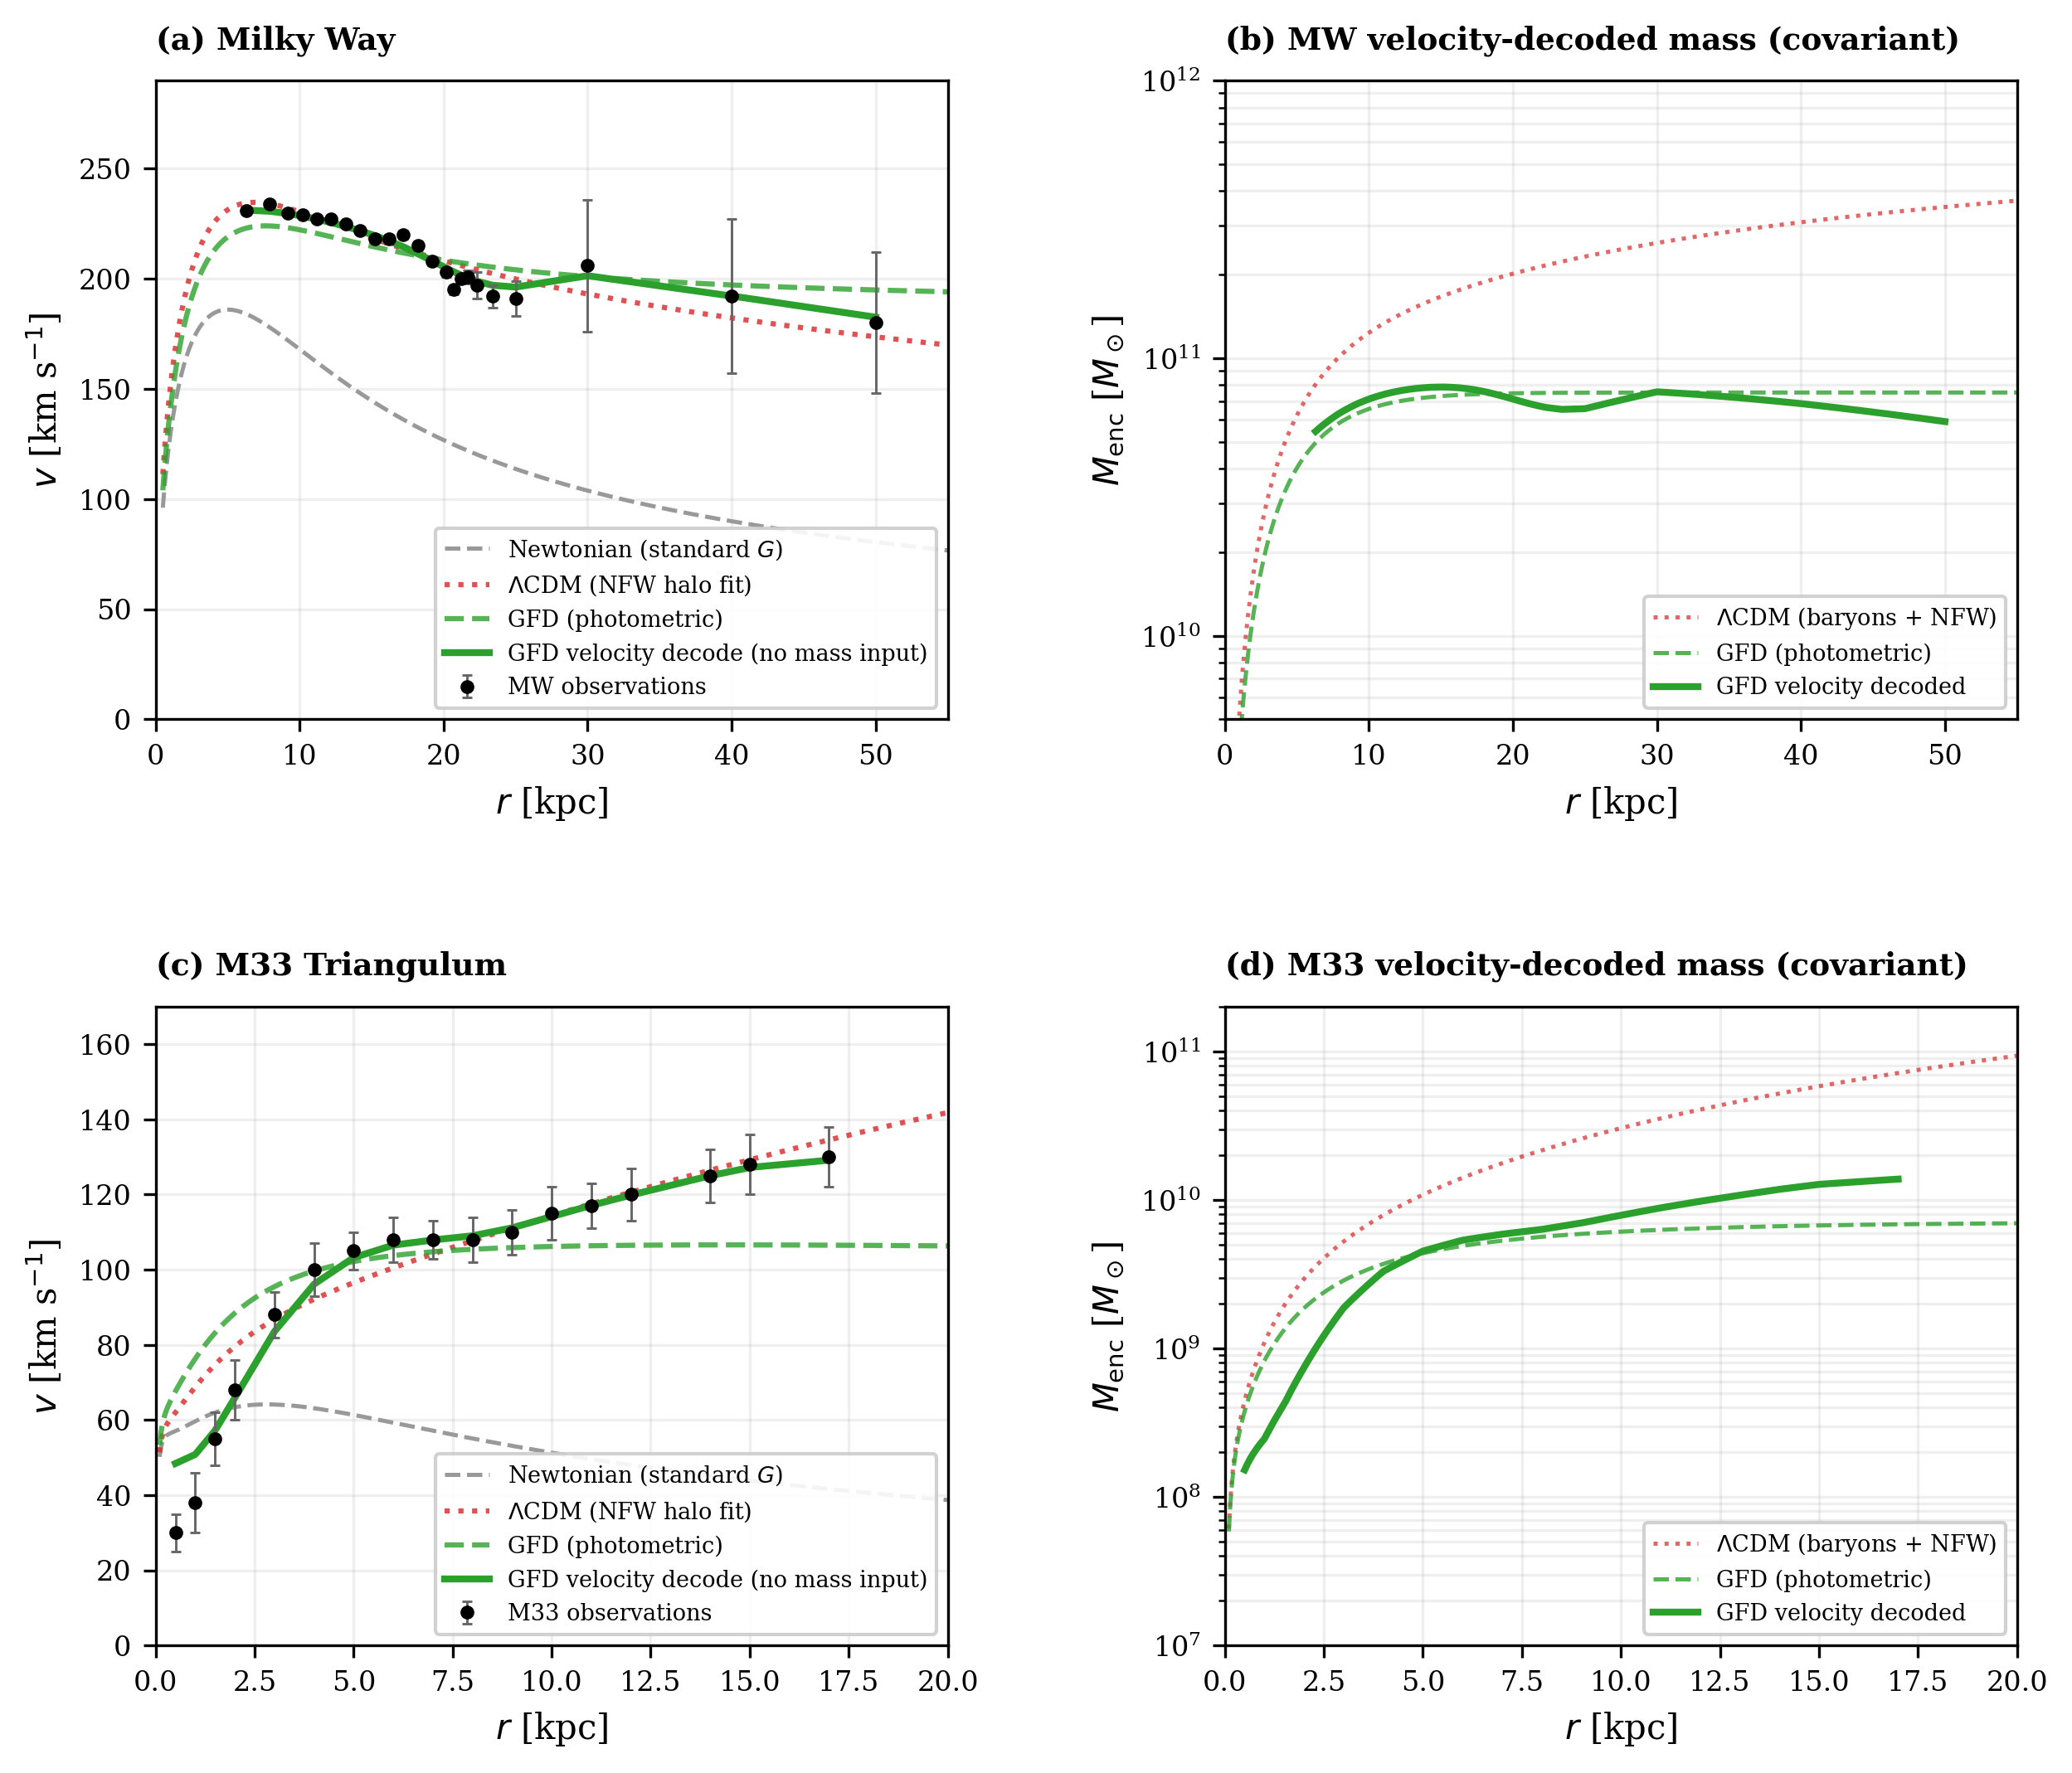
\includegraphics[width=\textwidth]{fig1_mw_m33}
\caption{\textbf{Four-panel comparison for the Milky Way and M33.}
(a) Milky Way rotation curve: observations (black), Newtonian from baryons with standard $G$ (grey dashed), $\Lambda$CDM with NFW halo (red dotted), GFD from photometric mass (green dashed), GFD velocity decode (green solid, from observed $v$ only).
(b) MW enclosed mass: $\Lambda$CDM baryons+NFW (red dotted), GFD photometric (green dashed), GFD velocity decoded (green solid). The solid green is the mass obtained by transforming $v(r)$ through the bidirectional covariant, not by fitting a halo.
(c) M33 rotation curve, same curve convention as (a).
(d) M33 enclosed mass, same as (b). Panels (b) and (d) show the mass each framework requires to produce the velocities in (a) and (c).}
\label{fig:1}
\end{figure*}

% ----------------------------------------------------------------------------
% 5. CONCLUSIONS
% ----------------------------------------------------------------------------
\clearpage

\begin{figure}[t]
\centering
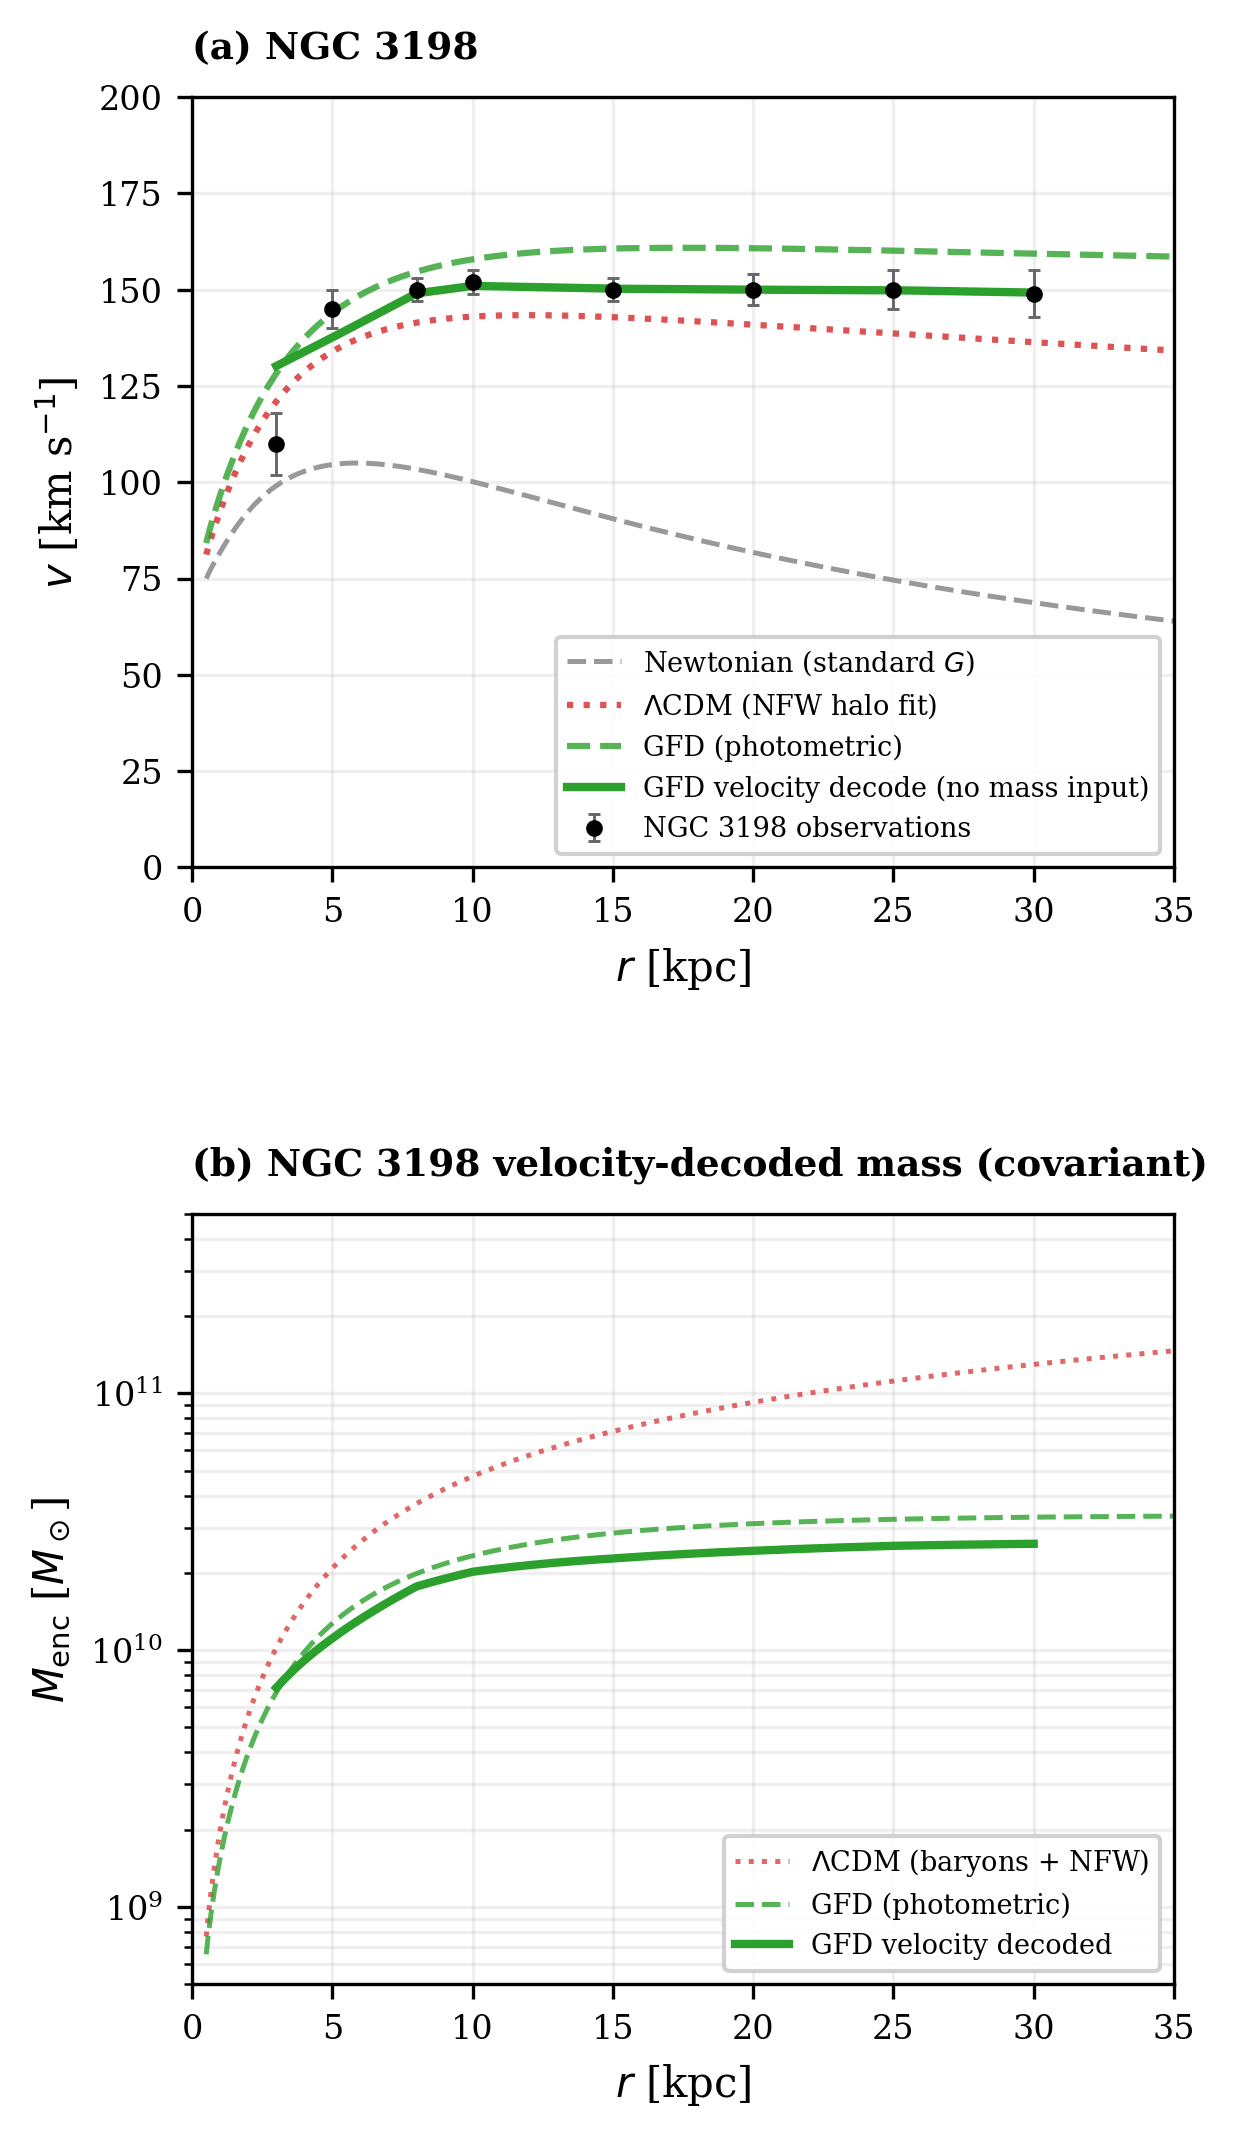
\includegraphics[width=\linewidth]{fig2_ngc3198}
\caption{NGC~3198. (a) Rotation curve: observations (black), Newtonian with standard $G$ (grey dashed), $\Lambda$CDM with NFW halo (red dotted), GFD photometric (green dashed), GFD velocity decode (green solid, from observed $v$ only). (b) Velocity-decoded enclosed mass (green solid) with $\Lambda$CDM and GFD photometric. Same Eq.~\ref{eq:Menc}, $G$, and $a_0$ as in Fig.~\ref{fig:1}; no fitted parameters.}
\label{fig:ngc3198}
\end{figure}

\null\vfill\newpage

\section{Conclusions}
\label{sec:conclusions}

The central result of this framework is a closed-form expression for the enclosed mass. From an observed rotation curve $v(r)$, Eq.~\ref{eq:Menc} gives
\begin{equation*}
M_{\mathrm{enc}}(r) = \frac{r\,v^4}{G\,(a_0\,r + v^2)}
\end{equation*}
with no iteration, no mass model, and no dark matter halo. We demonstrated this on the Milky Way and M33 (Fig.~\ref{fig:1}), where the decoded mass is consistent with known baryons within a factor of about two while $\Lambda$CDM requires several times more mass in halos to match the same velocities.

To test the framework further, we turn to NGC~3198, the canonical rotation-curve case in dark matter studies, with well-measured HI kinematics and independently inferred baryonic mass. As Fig.~\ref{fig:ngc3198} shows, the same equation, $G$, and $a_0$ yield a velocity-decoded mass (solid green) that tracks the known baryonic content and stays well below the $\Lambda$CDM enclosed mass (red dotted). No gravitational parameters are fitted: three galaxies, one formula, zero free parameters.

Because the velocity-to-mass inversion is algebraically exact and purely kinematic, the validity of these field equations can be falsified directly by observational data. Application of the pipeline to surveys such as SPARC \cite{Lelli16} would yield mass profiles testable against baryonic mass across many galaxies.

\section{Data and Code Availability}
\label{sec:data}
The rotation curve data used in this letter are from the published literature (McMillan 2017 for the Milky Way; Corbelli \& Salucci 2000 for M33; Begeman et al. 1991 for NGC~3198). Code to reproduce Figure~1 and the decoded mass profiles is provided in \texttt{generate\_letter\_figures.py}.

% ----------------------------------------------------------------------------
% REFERENCES (flow in column 1 under Data and Code)
% ----------------------------------------------------------------------------
\bibliography{letter,letterNotes}

\end{document}
